\documentclass[aspectratio=169]{beamer}
% Pacote de estilo da UDESC
\usepackage{style/udesc}
\usepackage{listings}
\usepackage{hyperref}
\setbeamertemplate{itemize items}[circle]
\usepackage[abnt-emphasize=bf,abnt-and-type=e,alf]{abntex2cite}%Citações ABNT


% Incluir arquivos da pasta figuras
\graphicspath{{./img/}}

\setbeamertemplate{frametitle continuation}{}

% aPacote de texto aleatório
\usepackage{lipsum}

\lstset{ 
	basicstyle=\footnotesize,        % the size of the fonts that are used for the code
	breakatwhitespace=false,         % sets if automatic breaks should only happen at whitespace
	breaklines=true,                 % sets automatic line breaking
	captionpos=b,                    % sets the caption-position to bottom
	deletekeywords={...},            % if you want to delete keywords from the given language
	escapeinside={\%*}{*)},          % if you want to add LaTeX within your code
	extendedchars=true,              % lets you use non-ASCII characters; for 8-bits encodings only, does not work with UTF-8
	firstnumber=0,                % start line enumeration with line 1000
	frame=single,	                   % adds a frame around the code
	keepspaces=true,                 % keeps spaces in text, useful for keeping indentation of code (possibly needs columns=flexible)
	language=Java,                 % the language of the code
	morekeywords={*,...},            % if you want to add more keywords to the set
	numbers=none,                    % where to put the line-numbers; possible values are (none, left, right)
	numbersep=0pt,                   % how far the line-numbers are from the code
	rulecolor=\color{black},         % if not set, the frame-color may be changed on line-breaks within not-black text (e.g. comments (green here))
	showspaces=false,                % show spaces everywhere adding particular underscores; it overrides 'showstringspaces'
	showstringspaces=false,          % underline spaces within strings only
	showtabs=false,                  % show tabs within strings adding particular underscores
	stepnumber=2,                    % the step between two line-numbers. If it's 1, each line will be numbered
	tabsize=1,	                   % sets default tabsize to 2 
	basicstyle=\fontsize{7}{8}\selectfont\ttstyle,
	keywordstyle=\color{blue},
	commentstyle=\fontsize{7}{8}\selectfont\ttstyle\color{gray},
	stringstyle=\color{orange},
}

% Início do documento
\begin{document}
\usetikzlibrary{positioning}
\usetikzlibrary{shadows.blur, trees}
\definecolor{greenudesc}{HTML}{01934A}
\usepgfmodule{animations}

%%
%%	Incluir \capa para os slides
%% 
\titulo{Produção Difrativa de}
\subtitulo{Mésons Vetoriais}
\newcommand{\autor}{Rodrigo Ribamar Silva do Nascimento}
\newcommand{\github}{github.com/physikices}
\newcommand{\email}{rodrigo.nascimento@edu.udesc.br}
\newcommand{\website}{}
\frase{2023 - IC Física de Partículas}
\universidade{Universidade do Estado de Santa Catarina}
\capa

\AtBeginSection[]{
	\begin{frame}<beamer>
		\frametitle{Seções}
		\tableofcontents[currentsection]
\end{frame}}
\section{Introdução}
\section{A Estrutura dos Hádrons}
\subsection{DIS}
\subsection{DIS no modelo de Pártons}
\subsection{As Equações de Evolução -- DGLAP}
\subsection{Parametrizações}
\section{Produção Difrativa de Mésons Vetoriais}
\subsection{Mésons}
\subsection{\textit{Hadronic Diffraction}}
\subsection{Seção de Choque p/  o Processo \texorpdfstring{${\gamma^{*}p\to pV}$}{lg}}
\section{Resultados}

% --------------------------------------------- %
% Introdução
% --------------------------------------------- %
\begin{frame}[plain]
	\tikzset{
		udesc greenBox/.style = {
			thin,
			blur shadow={
				shadow blur steps=10,
				shadow blur extra rounding=2pt, 
				shadow xshift=1pt
			},
			rectangle,
			minimum width=14em,
			minimum height=20mm,
			fill=greenudesc,
			text centered,
			anchor=base,
			inner sep=2ex
		},
	}
	\begin{tikzpicture}[remember picture,overlay]
		\node
			[udesc greenBox,yshift=-25pt,xshift=20pt] (box){}; 
		\node [right of = box, align=right,text=white] { {\LARGE Introdução}\\O Modelo Padrão};
	\end{tikzpicture}
\end{frame}
\begin{frame}{Introdução}
	\framesubtitle{O Modelo Padrão para a Física de Partículas}
	\begin{figure}[htb!]
		\centering
		\includegraphics[width=.58\linewidth]{tabela_modeloPadrao.png}
		\caption{Fonte: \cite{WORKMAN:2022}}
	\end{figure}	
\end{frame}

\begin{frame}[plain]
	\tikzset{
		udesc greenBox/.style = {
			thin,
			blur shadow={
				shadow blur steps=10,
				shadow blur extra rounding=2pt, 
				shadow xshift=1pt
			},
			rectangle,
			minimum width=18em,
			minimum height=20mm,
			fill=greenudesc,
			text centered,
			anchor=base,
			inner sep=2ex
		},
	}
	\begin{tikzpicture}[remember picture,overlay]
		\node
			[udesc greenBox,yshift=-25pt,xshift=15pt] (box){}; 
		\node [right of = box, align=right,text=white] { {\LARGE DIS}\\Deep Inelastic Scattering};
	\end{tikzpicture}
\end{frame}
% --------------------------------------------- %
% Deep Inelastic Scattering - DIS
% --------------------------------------------- %
\begin{frame}{A Estrutura dos Hádrons}
	\framesubtitle{Deep Inelastic Scattering}
	\begin{columns}
		\column{0.4\textwidth}
		\begin{center}
			\begin{tikzpicture}[thick,scale=1, every node/.style={transform shape}]
				\begin{feynhand}
	\vertex (a1) at (0,0){$\mathrm{e^{-}}$};
	\vertex (a2) at (2,0);
	\vertex (a3) at (4,1);
	\vertex (b) at (2.5,-1.2);
	\vertex (a4) at (b);
	\uncover<2->{\vertex (a5) at (0,-1.25){$p$};}
	\uncover<3->{\vertex (a6) at (4.5,-1.25){$X$};}

	\propag [fer,  mom={$k$}] (a1) to (a2);
	\uncover<3->{\propag [fer,  mom={$k^{\prime}$}] (a2) to (a3);
	\propag [pho] (a2) to [edge label=$\gamma^{*}$] (a4);}
	\uncover<2->{\propag [fer] (a5) to (2.5,-1.25);}
	\uncover<3->{
		\propag [fer] (2.5,-1.) to (4,-1);
		\propag [fer] (2.5,-1.25) to (4,-1.25);
		\propag [fer] (2.5,-1.5) to (4,-1.5);
	}
	\uncover<2->{\vertex [blob,fill=greenudesc!40!white] at (2.5, -1.2) (c) {};}
\end{feynhand}

			\end{tikzpicture} 
		\end{center}
		\column{0.6\textwidth}
		\only<4-7>{
			\begin{align*}
				\frac{d \sigma}{d \Omega dE^{\prime}}\Bigg|_{ep\to eX}=&
				\only<4>{\left(\frac{\alpha^{2}}{4E^{2}\sin^{4}\theta/2}\right)\frac{1}{4EE^{\prime}}L^{\mu \nu}_{(L)}W^{(H)}_{\mu \nu}}
				\only<5-8>{\left(\frac{4 \alpha^{4}E^{\prime 2}}{q^{4}}\right)\left[2\sin^{2}\frac{\theta}{2}W_{1}(\nu,Q^{2})+\right. \\& \left. \quad +\cos^{2}\frac{\theta}{2}W_{2}(\nu, Q^{2})\right]}
			\end{align*}
		}
		\only<8>{
			\begin{align*}
				\frac{d \sigma}{d\Omega dE^{\prime}}&=\frac{1}{s+u}\left(\frac{4 \pi \alpha^{2}}{s^{2}t^{2}}\right)\times \\ &\quad \times \left[-(s+u)t\color{magenta}{MW_{1}(\nu, Q^{2})} \color{black}{+}\right.\\ & \left. \qquad\qquad -us\color{magenta}{\nu W_{2}(\nu,Q^{2})}\color{black}\right]
			\end{align*}	
		}
	\end{columns}
	\only<6->{
		\begin{equation*}
			\left.\begin{aligned}
					s & \equiv (p+k)^{2}=E^{2}_{cm},\\
					t &\equiv (k-k^{\prime})=-Q^{2},\\
					u &\equiv (k-p_{x})^{2}
				\end{aligned}
			\right\}
			\only<7->{\qquad s+t+u=M^{2}+W^{2}}
		\end{equation*}
	}
\end{frame}
% --------------------------------------------- %
% O DIS no Modelo de Partons 
% --------------------------------------------- %

\begin{frame}{A Estrutura dos Hádrons}
	\framesubtitle{DIS no Modelo de Partons}
	\only<1-3>{
		\begin{block}{Stanford Linear Accelerator - SLAC (1960)}
			\begin{subequations}
				\begin{align*}
					\lim_{Q^{2},\nu\to \infty}\color{magenta}{MW_{1}(\nu, Q^{2})}&\approx F_{1}(x)\\
					\lim_{Q^{2},\nu\to \infty}\color{magenta}{\nu MW_{2}(\nu, Q^{2})}&\approx F_{2}(x)\only<2-3>{\implies x\equiv \frac{Q^{2}}{2M \nu}}
				\end{align*}
				\only<3>{
					\begin{align*}
						\sigma^{\gamma^{*}p}_{L}&=\frac{4 \pi^{2} \alpha}{Q^{2}}\left[F_{2}(x,Q^{2})-2xF_{1}(x,Q^{2})\right]\\
						\sigma^{\gamma^{*}p}_{T}&=\frac{4 \pi^{2} \alpha}{Q^{2}}\left[2xF_{1}(x,Q^{2})\right]
					\end{align*}
				}
			\end{subequations}
		\end{block}
	}

	\only<4->{
		\only<4>{
			\begin{center}
				\begin{figure}[htb!]
					\centering
					\includegraphics[width=.45\linewidth]{f2vsx.pdf}
					\caption{Fonte: \cite{WORKMAN:2022}}
				\end{figure}
			\end{center}
		}
		\only<5->{
			\begin{columns}
				\column{0.5\textwidth}
				\begin{tikzpicture}[thick,scale=1.0, every node/.style={transform shape}]
					\begin{feynhand}
	\vertex (a) {$\mathrm{e}^{-}$};
	\vertex [right=of a] (b);
	\vertex [below right=of b] (c);
	\vertex [above right=of b] (f1) {$\mathrm{e}^{-}$};
	\vertex [right=of c] (d){$\xi p+q$};
	

	\propag [fer, mom={$k$}] (a) to (b);
	\propag [fer, mom={$k^{\prime}$}] (b) to (f1);
	\propag [pho] (b) to [edge label=$\gamma^{*}(\nu)$] (c);
	\propag [fer] (c) to (d);

	\vertex (g1) at (1.35,-1.7);
	\vertex (g12) at (3.4,-1.7);

	\vertex (g2) at (1.35,-1.9);
	\vertex (g21) at (4.4,-1.9){$X(1-\xi p)$};

	\vertex (g3) at (1.35,-2.1);
	\vertex (g31) at (3.4,-2.1);

	\propag [fer] (g1) to (g12);
	\propag [fer] (g2) to (g21);
	\propag [fer] (g3) to (g31);

	% \propag [fer] (p) to (e);
	\vertex [blob,fill=red!50!white, below=1.5cm of b] (p){};
	\vertex [left=.8cm of p] (p1) {$p$};
	% \vertex [right=1.6cm of p] (e);

	\propag [fer] (p) to (c);
	\propag [fer] (p1) to (p);

\end{feynhand}

				\end{tikzpicture}
				\column{0.5\textwidth}
				\only<5->{
					\only<5-11>{
						\begin{alert}{Função Densidade Partônica (PDF):}
							\begin{align*}
								\sum_{q} \xi_{q}p&=p\\
								\uncover<6->{
								m_{q}^{2}&=(\xi p+q)^{2}=0\uncover<7->{\implies \boxed{\xi= x}}\\
							}
							\only<8>{
								\sigma^{\gamma^{*}p}&=\sum_{q}\int\limits_{0}^{1}\,d{\xi}f_{q}(\xi)\hat{\sigma}^{\gamma^{*}p}_{\color{greenudesc}{L},\color{blue!50!black}{T}}\\
							}
							\only<9-10>{
								\color{greenudesc}{\sigma_{L}^{\gamma^{*}p}(x,Q^{2})}&\color{greenudesc}{=0}\only<10>{\implies \\& \color{magenta}{F_{2}(x,Q^{2})=2xF_{1}(x,Q^{2})}}\\
								\color{blue!50!black}{\sigma^{\gamma^{*}p}_{T}(x,Q^{2})}&\color{blue!50!black}{=\frac{4 \pi^{2} \alpha}{Q^{2}}2xF_{1}(x,Q^{2})}
							}
							\only<11>{
								\sigma^{\gamma^{*}p}&=\frac{4 \pi^{2} \alpha}{Q^{2}}\color{magenta}{\sum_{q}\int\limits_{0}^{1}\,d{\xi}f_{q}(\xi)e^{2}_{q} \delta\left(1-\frac{x}{\xi}\right)}\\
								\sigma^{\gamma^{*}p}&=\frac{4 \pi^{2} \alpha}{Q^{2}}\color{magenta}{\sum_{q}e_{q}^{2}xf_{q}(x)}
							}
						\end{align*}															
					\end{alert}
				}
				\only<12>{
					\begin{block}{Resultados Experimentais \cite{RODRIGO:2016,LUIS:2014}}
						\begin{align*}
							f_{u}&=\int\limits_{0}^{1}xu(x)\,d{x}=0.36\\
							f_{d}&=\int\limits_{0}^{1}xd(x)\,d{x}=0.18\\
									 &\boxed{\approx 54\%}\to \text{quarks $u$ e $d$}
						\end{align*}						
					\end{block}
				}
				\only<13->{
					\begin{center}
						\begin{tikzpicture}
							\node[squarednode] (main) {\textbf{E AGORA??}};
							\only<14>{
								\node[squarednode, below=of main] (second) {$F_{i}(x)\to F_{i}(x,Q^{2})$};
								\draw[->] (main) -- (second) node [above right=17pt, fill=white] {via QCD};
							}
						\end{tikzpicture}
					\end{center}
				}
			\end{columns}
		}
	}
}
\end{frame}
% --------------------------------------------- %
% --------------------------------------------- %[FRAME DESLOCADO]
\begin{frame}{A Estrutura dos Hádrons}
 	\framesubtitle{QED}
	\begin{columns}
		\column{0.5\textwidth}
		A constante de acoplamento $\alpha_{s}$
		
		\only<1>{
			\begin{itemize}
				\item Determina a intensidade da força de interação forte;
				\item Depende da distância ou da escala de momento entre as partículas;
				\item É obtida por meio da equação do grupo de renormalização;
			\end{itemize}
		}
		\only<2>{
			\begin{align*}
				\frac{d \alpha_{s}(Q^{2})}{dt}&=\beta(\alpha_{s}(Q^{2}))\\
				t&=\log \left(\frac{Q^{2}}{\mu^{2}}\right)\\
				\beta(\alpha_{s})&=\mu^{2}\frac{d \alpha_{s}}{d{\mu^{2}}}
			\end{align*}
			A função $\beta$ expressa a dependência de $\alpha_{s}$ na escala de energia de algum processo, e é dada pela expansão pertubativa $\beta(\alpha_{s})=-\alpha_{s}^{2}[b_{0}+b_{1} \alpha_{s}+\mathcal{O}(\alpha_{s}^{2})]$
		}

		\column{0.5\textwidth}
		\begin{figure}[htb!]
			\centering
			\includegraphics[width=.6\textwidth]{img/alphas-v-Q-2021.pdf}
			\caption{Evolução da constante de acoplamento forte em função de $Q$. Fonte: \cite{WORKMAN:2022}}
		\end{figure} 
	\end{columns}
	
	
\end{frame}
% --------------------------------------------- %
% As Equações DGLAP
% --------------------------------------------- %
\begin{frame}[plain]
	\tikzset{
		udesc greenBox/.style = {
			thin,
			blur shadow={
				shadow blur steps=10,
				shadow blur extra rounding=2pt, 
				shadow xshift=1pt
			},
			rectangle,
			minimum width=18em,
			minimum height=20mm,
			fill=greenudesc,
			text centered,
			anchor=base,
			inner sep=2ex
		},
	}
	\begin{tikzpicture}[remember picture,overlay]
		\node
			[udesc greenBox,yshift=-25pt,xshift=15pt] (box){}; 
		\node [right of = box, align=right,text=white] { {\LARGE DGLAP}\\As Equações de Evolução};
	\end{tikzpicture}

\end{frame}
\begin{frame}{DGLAP}
	\framesubtitle{Remodelando as Funções de Estrutura}
	\begin{tikzpicture}[thick, scale=1, every node/.style={transform shape}]
		\begin{feynhand}
	\vertex (v1) at (1.3, -.9);
	\vertex [below=1.3of v1] (v2);

	\node (a1) at (0,0){$\mathrm{e}^{-}$};
	\node (a2) at (2,.0);
	\node[orange] (a3) at (0,-3.3){$q$};
	\only<2->{
		\node[squarednode] (a3) at (0,-3.3){$\color{orange}{q}$};
		\node[squarednode] (a3b) at (6, -4){$q(x)\implies q(x,Q^{2})=q(x)+\Delta q(x,Q^{2})$};
		\draw[->] (a3.south) .. controls +(down:7mm) and +(left:7mm) .. (a3b.west);
	}
	\node (a4) at (2,-3.3);


	\propag[pho] (v1) to [edge label=$\gamma(Q^{2})$] (v2);
	\propag[fer] (a1) to (v1);
	\propag[fer] (v1) to (a2);
	\propag[fer, orange] (a3) to [edge label=$\xi p$] (v2);
	\propag[fer] (v2) to (a4);

\end{feynhand}

		\only<3-7>{
			\node[roundnode] (a1) at (8.5,-4){$\Delta q(x,Q^{2})$};
			\only<4-5>{
				\node[above left=of a1] (a2){
						\begin{tikzpicture}[decoration={markings, mark= at position 0.5 with {\arrow{latex}}}] 
							\begin{feynhand}
	\vertex (v1);
	\vertex[right=2cm of v1] (v2);

	\propag[pho] (v1) to [edge label=$\gamma$] (-.5,1);
	\draw[postaction={decorate}] (-.5,-1) to [edge label=$q$] (v1);
	\draw[postaction={decorate}] (v1) to [edge label=$z(yp)-xp$] (2,0);
	\propag[glu] (v2) to [edge label=$g$] (2.5,-1);
	\draw[postaction={decorate}] (v2) to [edge label=$q$] (2.5,1);
\end{feynhand}

 
% \draw [postaction={decorate}] (0,0) -- (2,2); 


						\end{tikzpicture}
					};
					\only <4-5>{
						\draw[->](a1.north) .. controls +(up:7mm) and +(down:7mm) .. (a2.south);
					}
				}
				\only<5>{
					\node[right=2cm of a2] (a3){
						\begin{tikzpicture}[decoration={markings, mark= at position 0.5 with {\arrow{latex}}}] 
							\begin{feynhand}
	\vertex (v1);
	\vertex[below=of v1] (v2);

	\propag[pho] (v1) to [edge label=$\gamma$] (-1,1);
	\draw[postaction={decorate}] (v1)  to [edge label=$q$] (1,1);
	\draw[postaction={decorate}] (v2) to (v1);
	\draw[postaction={decorate}] (-1,-2) to [edge label=$q$] (v2);
	\propag[glu] (1,-2) to [edge label=$g$] (v2);
\end{feynhand}

						\end{tikzpicture}
					};
					\only <5>{
						\draw[->](a1.north) .. controls +(up:7mm) and +(down:7mm) .. (a3.south);
					}
				}
				\only<6->{
					\node[level 3, above left=of a1] (a2) {$\displaystyle{\frac{\alpha_{s}t}{2 \pi}\int\limits_{x}^{1}\,\frac{d{y}}{y}q(y)P_{qq}\left(\frac{x}{y}\right)}$}; 
					\draw[->](a1.north) .. controls +(up:7mm) and +(down:7mm) .. (a2.south);

					\only<7>{
						\node[level 3, right=of a2] (a3) {$\displaystyle{t=\ln \left(\frac{Q^{2}}{\mu^{2}}\right)}$};
						\draw[->](a2.east) .. controls +(right:7mm) and +(left:7mm) .. (a3.west);
					}
				}
			}
		\end{tikzpicture}

	\end{frame}

	\begin{frame}{DGLAP}
		\framesubtitle{Processo $\gamma g\to q \bar{q}$}
		\only<1>{
			\begin{tikzpicture}[thick, scale=1, every node/.style={transform shape}]
				\node (a1){
						\begin{tikzpicture}[decoration={markings, mark= at position 0.5 with {\arrow{latex}}}] 
							\begin{feynhand}
	\vertex (v1);	
	\vertex[below=1.5cm of v1] (v2);

	\draw[postaction={decorate}] (v2) to (v1);
	\draw[postaction={decorate}] (v1) to [edge label=$q$] (1,.3);
	\draw[postaction={decorate}] (1,-1.7) to [edge label=$\bar{q}$] (v2);

	\propag[pho] (v1) to [edge label=$\gamma(Q^{2})$] (-1,.5);
	\propag[glu] (v2) to [edge label=$g$] (-1,-2);
\end{feynhand}

						\end{tikzpicture}
					};
					\node[level 3, right=of a1] (a2){$\displaystyle{\ldots g(y)P_{qg}\left(\frac{x}{y}\right)}$};
					% \only <2>{
					% 	\draw[->](a1.north) .. controls +(up:7mm) and +(down:7mm) .. (a3.south);
					% }
				\end{tikzpicture}
			}
		\end{frame}

		\begin{frame}{DGLAP}
			\framesubtitle{Funções de splitting}
			\begin{tikzpicture}[thick, scale=1, every node/.style={transform shape}]
				\node (a1){
						\begin{tikzpicture}[decoration={markings, mark= at position 0.5 with {\arrow{latex}}}]
							\begin{feynhand}
	\vertex (v1);		

	\draw[postaction={decorate}] (-1,0) to [edge label=$q(y)$] (v1);
	\draw[postaction={decorate}] (v1) to [edge label=$q(x)$] (1,1);
	\propag[glu] (v1) to [edge label=$g(y-x)$] (1,-1);
\end{feynhand}
	
						\end{tikzpicture}
					};
					\node[right=.2cm of a1] (a2){
						\begin{tikzpicture}[decoration={markings, mark= at position 0.5 with {\arrow{latex}}}]
							\begin{feynhand}
	\vertex (v1);		

	\draw[postaction={decorate}] (-1,0) to [edge label=$q(y)$] (v1);
	\draw[postaction={decorate}] (v1) to [edge label=$q(y-x)$] (1,-1);
	\propag[glu] (v1) to [edge label=$g(x)$] (1,1);
\end{feynhand}
	
						\end{tikzpicture}
					};
					\node[right=.2cm of a2] (a3){
						\begin{tikzpicture}[decoration={markings, mark= at position 0.5 with {\arrow{latex}}}]
							\begin{feynhand}
	\vertex (v1);		

	\propag[glu] (-1,0) to [edge label=$g(y)$] (v1);
	\draw[postaction={decorate}] (1,-1) to [edge label=$q(y-x)$] (v1);
	\draw[postaction={decorate}] (v1) to [edge label=$q(x)$] (1,1);
\end{feynhand}
	
						\end{tikzpicture}
					};
					\node[right=.2cm of a3] (a4){
						\begin{tikzpicture}[decoration={markings, mark= at position 0.5 with {\arrow{latex}}}]
							\begin{feynhand}
	\vertex (v1);		

	\propag[glu] (-1,0) to [edge label=$g(y)$] (v1);
	\propag[glu] (1,-1) to [edge label=$g(y-x)$] (v1);
	\propag[glu] (1,1) to [edge label=$g(x)$] (v1);
\end{feynhand}
	
						\end{tikzpicture}
					};
					\only<2->{
						\node[level 3,below=.3cm of a1]{$\displaystyle{P_{qq}\left(\frac{x}{y}\right)}$};
						\node[level 3,below=.3cm of a2](b0){$\displaystyle{P_{gq}\left(\frac{x}{y}\right)}$};
						\node[level 3,below=.3cm of a3](b1){$\displaystyle{P_{qg}\left(\frac{x}{y}\right)}$};
						\node[level 3,below=.3cm of a4]{$\displaystyle{P_{gg}\left(\frac{x}{y}\right)}$};
					}
					\only<3>{
						\node[squarednode,below=.3cm of b0]{$\displaystyle{\frac{dq(x,t)}{dt}=\frac{\alpha_{s}}{2 \pi}\int\limits_{x}^{1}\left[q(x,t)P_{qq}\left(\frac{x}{y}\right)+g(x,t)P_{qg}\left(\frac{x}{y}\right)\right]\,\frac{d{y}}{y}}$};
					}
					\only<4>{
						\node[squarednode,below=.3cm of b1]{$\displaystyle{\frac{dg(x,t)}{dt}=\frac{\alpha_{s}}{2 \pi}\int\limits_{x}^{1}\left[\sum_{j}q_{j}(x,t)P_{qg}\left(\frac{x}{y}\right)+g(x,t)P_{gg}\left(\frac{x}{y}\right)\right]\,\frac{d{y}}{y}}$};
					}
				\end{tikzpicture}
			\end{frame}

			% --------------------------------------------- %

			% --------------------------------------------- %
			% Parametrizações das PDFs
			% --------------------------------------------- %
			\begin{frame}[plain]
				\tikzset{
					udesc greenBox/.style = {
						thin,
						blur shadow={
							shadow blur steps=10,
							shadow blur extra rounding=2pt, 
							shadow xshift=1pt
						},
						rectangle,
						minimum width=18em,
						minimum height=20mm,
						fill=greenudesc,
						text centered,
						anchor=base,
						inner sep=2ex
					},
				}
				\begin{tikzpicture}[remember picture,overlay]
					\node
						[udesc greenBox,yshift=-25pt,xshift=15pt] (box){}; 
					\node [right of = box, align=right,text=white] { {\LARGE Parametrizações}\\Distribuições partônicas};
				\end{tikzpicture}
			\end{frame}

			\begin{frame}{Parametrizações partônicas}
				\framesubtitle{Grupos}
				\begin{figure}[htb!]
					\centering
					\includegraphics[width=.55\linewidth]{grupos_parametrizacoes.png}
					\caption{Distribuições gluônicas em função da fração de momentum para a escala $Q^{2}=2,4\mathrm{GeV}^{2}$. Fonte: \cite{LUIS:2014}}
				\end{figure}

			\end{frame}

			% --------------------------------------------- %

			% --------------------------------------------- %
			% Produção Difrativa
			% --------------------------------------------- %
			\begin{frame}[plain]
				\tikzset{
					udesc greenBox/.style = {
						thin,
						blur shadow={
							shadow blur steps=10,
							shadow blur extra rounding=2pt, 
							shadow xshift=1pt
						},
						rectangle,
						minimum width=18em,
						minimum height=20mm,
						fill=greenudesc,
						text centered,
						anchor=base,
						inner sep=2ex
					},
				}
				\begin{tikzpicture}[remember picture,overlay]
					\node
						[udesc greenBox,yshift=-25pt,xshift=15pt] (box){}; 
					\node [right of = box, align=right,text=white] { {\LARGE Mésons Vetoriais}\\Produção difrativa};
				\end{tikzpicture}
			\end{frame}

			\begin{frame}{Mésons Vetoriais}
				\framesubtitle{Propriedades}
				\begin{table}[!ht]
					\resizebox{\textwidth}{!}{%
						\begin{tabular}{|c|c|c|c|c|c|}
							\hline
							\textbf{Méson} & \textbf{Conteúdo de Quarks} & \textbf{Carga} & \textbf{Massa} & \textbf{Tempo de Vida} & \textbf{Principais Decaimentos} \\ \hline
							$\rho$ & $u\bar{d},(u\bar{u}-d\bar{d})\sqrt{2},d\bar{u}$ & 1,0,-1 & 775,5 & $4\times 10^{-24}$ & $\pi\pi$ \\ \hline
							$K^{*}$ & $u\bar{s},d\bar{s},s\bar{d},s\bar{u}$ & 1,-1 & 894 & $1\times 10^{-23}$ & $K\pi$ \\ \hline
							$\omega$ & $(u\bar{u}+d\bar{d})\sqrt{2}$ & 0 & 782,6 & $8\times 10^{-23}$ & $\pi\pi\pi ,\pi\gamma$ \\ \hline
							$\psi$ & $c\bar{c}$ & 0 & 3097 & $7\times 10^{-21}$ & $e^{+}e^{-},\mu^{+}\mu^{-}\pi ,5\pi, 7\pi$ \\ \hline
							$D^{*}$ & $c\bar{d},c\bar{u},u\bar{c},d\bar{c}$ & 1,0,-1 & 2008 & $3\times 10^{-21}$ & $D\pi,D\gamma$ \\ \hline
							$\Upsilon$ & $b\bar{b}$ & 0 & 9460 & $1\times 10^{-20}$ & $e^{+}e^{-},\mu^{+}\mu^{-}\pi ,\tau^{+}\tau^{-}$ \\ \hline
						\end{tabular}%
					}
					\caption{Algumas propriedades físicas dos mésons vetoriais. Fonte: \cite{LUIS:2014}}
				\end{table}
			\end{frame}

			\begin{frame}{Hadronic Diffraction}
				\framesubtitle{Definição}
				\only<1->{
					\begin{tikzpicture}
						\node[squarednode, draw, align=center, text width=.9\textwidth] (cite01) {
								\begin{minipage}{\textwidth}
									[\dots]Good and Walker who in 1960, wrote: \emph{``...A phenomenal is predicted in which a high energy particle beam undergoing diffraction scattering from a nucleous will acquire components corresponding to various products of the virtual dissocitions of the incidente particle... These diffraction-produced system would have a characteristic extremelt narrow distribution  in transverse momentum  and would have the same quantum numbers of the initial particle...''}

									For the sake of definiteness, we will say that \emph{``every reaction in which no quantum numbers are exchange between high energy colliding particles is domined asympthotically by diffraction.''} \cite{PREDAZZI:1998}
								\end{minipage}
							};
					\end{tikzpicture}
				}
			\end{frame}

			\begin{frame}{Mésons Vetoriais}
				\framesubtitle{Fotoprodução do Méson $J/\psi$} 

				\begin{tikzpicture}
					\setlength{\abovedisplayskip}{0pt}
					\setlength{\belowdisplayskip}{0pt}
					\only<3->{
						\node[rectangle,
							fill = magenta!20,
							minimum width = .8cm, 
							minimum height = 1.8cm] (e) at (2.42,.9) {};
					}
					\input{img/jpsi_diagram-b.tex}
					\only<4-5>{
						\node [squarednode, draw, align=center] at (6.6,3) (example) {\emph{c. sec.} - HERA:\\\cite{LUIS:2014}};
						\node [mathnode, right=.5cm, text width=3.6cm] (eq1) at (example.east) {
								\begin{minipage}{\textwidth}
									\begin{align*}
										\sigma^{\gamma p\to Vp}(W^{2})&\sim W^{0,2}\\
										V\to \rho,\omega,&\text{ e } \phi
									\end{align*}
									\centering
									(Aumenta)
								\end{minipage}
							};
						\draw [->, line width=1pt] (example) -- (eq1);
						\only<5>{
							\node [squarednode, draw, align=center, text width=3.6cm, below=2.5cm] (txt) at (eq1.south){
									\begin{minipage}{\textwidth}
										\centering
										Este aumento é ainda mais significatico para o processo $J/\psi$
									\end{minipage}
								};
							\draw [->, line width=1pt] (eq1) -- (txt);
							\node [mathnode, draw, align=center, text width=5cm, left=2cm] (txt2) at (txt.west){
									\begin{minipage}{\textwidth}
										\begin{align*}
											\frac{d\sigma^{\gamma g\to c\bar{c}}}{dt}\Bigg|_{t=0} \propto \left[\bar{x}g(\bar{x},\bar{Q^{2}})\right]^{2}
										\end{align*}
									\end{minipage}
								};
							\draw [->, line width=1pt] (txt) to [edge label=(pQCD)] (txt2);
						}

					}
					\only<6-7>{
						\node [mathnode, draw, align=center, text width=6cm, right=4.5cm] (main) at (e.north){
								\begin{minipage}{\textwidth}
									\begin{align*}
										\displaystyle\frac{d\sigma^{\gamma g\to c\bar{c}}}{dt}\Bigg|_{t=0} \propto \left[\alpha_{s}x_{P}g(x_{P},\bar{Q^{2}})\right]^{2}
									\end{align*}
								\end{minipage}
							};
						\node [squarednode, draw, align=center, text width=6cm, below=.5cm] (sec) at (main.south){
								\begin{minipage}{\textwidth}
									\begin{enumerate}
										\item $x_{P}$ -- fração de momentum portada pelo do próton
										\item $g(x_{P},\bar{Q^{2}})$ -- distrib. de glúons a $Q^{2}$ efetivo
										\item $\alpha_{s}$ -- constante de acoplamento \textit{strong}
									\end{enumerate}
								\end{minipage}
							};
						\only<7>{
							\node [mathnode, draw, align=center, text width= 3cm, left=1cm] (thrd) at (sec.west){
									\begin{minipage}{\textwidth}
										\begin{align*}
											\bar{Q^{2}}&=\frac{Q^{2}+M_{V}}{4}
										\end{align*}
									\end{minipage}
								};
						}
					}
				\end{tikzpicture}
			\end{frame}

			\begin{frame}{Mésons Vetoriais}
			\framesubtitle{Amplitude de Espalhamento}
			\begin{tikzpicture}
				\node (main) at (0,0) {
						\begin{tikzpicture}
							\begin{feynhand}
	% proton
	\vertex(p1) {$P$};
	\vertex[right=2cm of p1](blob) {};
	\vertex[right=2cm of blob](p2) {$P^{\prime}$};

	\propag[fer] (p1) -- (blob);
	\propag[fer] (blob) -- (p2);

	% eletron
	\vertex[above=2cm of p1] (e1) {$\mathrm{e}^{-}$};
	\vertex[right=1cm of e1] (e2);
	\vertex[above right=1cm of e2] (e3);

	\propag[fer] (e1) -- (e2);
	\propag[fer] (e2) -- (e3);

	% foton
	\vertex[below right=1cm of e2] (f1);

	% gluons
	\vertex[left=.1cm of blob] (g1);
	\vertex[right=.1cm of blob] (g2);
	\vertex[above=1.77cm of g1] (g3);
	\vertex[above=2.49cm of g2] (g4);\node[left=.5cm of f1]{$q(l^{\prime})$};

	\propag[glu,red] (g1) to [edge label=$g(k)$] (g3);
	\propag[glu,orange] (g2) to node [right] {$g(k^{\prime})$} (g4);

	% loop
	\vertex[above=2cm of blob] (center_loop);
	\vertex[right=.8cm of center_loop] (l1);
	\vertex[left=.8cm of center_loop] (l2);

	\propag[fer] (l1) to [half right,looseness=.8] (l2);
	\propag[fer] (l2) to [half right,looseness=.8] (l1);

	% j/psi
	\vertex[right=2cm of center_loop] (pivot);
	\vertex[above=.01cm of pivot] (pivot-a){$\bar{c}$};
	\vertex[below=.01cm of pivot] (pivot-b){$c$};

	\propag[fer] (pivot-a) to ++(-1.42cm,0);
	\propag[antfer] (pivot-b) to ++(-1.35cm,0);

	


	\vertex[blob, fill=gray] at (blob) {};
	\propag[pho] (e2) to [edge label=$\gamma$] (l2);
	\draw [decoration={brace}, decorate] (pivot-a.north east) -- (pivot-b.south east)
          node [pos=0.5, right] {$J/\psi$};
\end{feynhand}

						\end{tikzpicture}
					};
					\only<1->{
						\node[mathnode, draw, align=center, text width=6.9cm, right=2.9cm] (amplitude_espalhamento) {
							\begin{minipage}{\textwidth}
									\begin{align*}
										A_{T}=&-4 \pi^{2}i \alpha_{s}W^{2}\int\,\frac{dk^{2}}{k^{4}}\left(\color{red}{\frac{1}{l^{2}-m_{c}^{2}}}\color{black}{+}\right. \\ & \left. \quad  - \color{orange}{\frac{1}{l^{\prime 2}-m_{c}^{2}}}\color{black}\right)f(x_{P},k^{2})e_{c}g_{\psi}M_{\psi}
									\end{align*}
							\end{minipage}
						};
						\only<2>{
							\node[mathnode, draw, align=center, text width=6cm, below=.5cm] (sec_choque) at (amplitude_espalhamento.south){
								\begin{minipage}{\textwidth}
									\begin{align*}
										\frac{d \sigma_{T}^{\gamma^{(*)}p\to \psi p}}{dt}&=\frac{1}{16 \pi W^{4}}\abs{A_{T}}^{2}	
									\end{align*}
								\end{minipage}
							};
						}
						\only<3->{
							\node[level 3, draw, align=center, text width=12cm, below=2.5cm of e] (sc_total) {
								\begin{minipage}{\textwidth}
									\begin{align*}
										\frac{d \sigma_{T}^{\gamma^{(*)}p\to \psi p}}{dt}\Bigg|_{t=0} &= \frac{16 \Gamma_{e^{+}e^{-}}^{\psi}M_{\psi}^{3} \pi^{3}}{3 \alpha_{em}\left(Q^{2}+M^{2}_{\psi}\right)^{4}}\left[\alpha_{s}(\bar{Q}^{2})x_{P}g(x_{P},\bar{Q^{2}})\right]^{2}\left(1+\frac{Q^{2}}{M_{\psi}}\right)
									\end{align*}
								\end{minipage}
							};
						}
					}
			\end{tikzpicture}
				
								
				
			\end{frame}

			% --------------------------------------------- %

			% --------------------------------------------- %
			% Resultados
			% --------------------------------------------- %
			\begin{frame}[plain]
				\tikzset{
					udesc greenBox/.style = {
						thin,
						blur shadow={
							shadow blur steps=10,
							shadow blur extra rounding=2pt, 
							shadow xshift=1pt
						},
						rectangle,
						minimum width=15em,
						minimum height=20mm,
						fill=greenudesc,
						text centered,
						anchor=base,
						inner sep=2ex
					},
				}
				\begin{tikzpicture}[remember picture,overlay]
					\node
						[udesc greenBox,yshift=-25pt,xshift=15pt] (box){}; 
					\node [right of = box, align=right,text=white] { {\LARGE Resultados}\\Análise Numérica};
				\end{tikzpicture}
			\end{frame}
			
			\begin{frame}{Resultados}
			\framesubtitle{Análise Numérica}
				\only<1>{
					\begin{figure}[htb!]
						\centering
						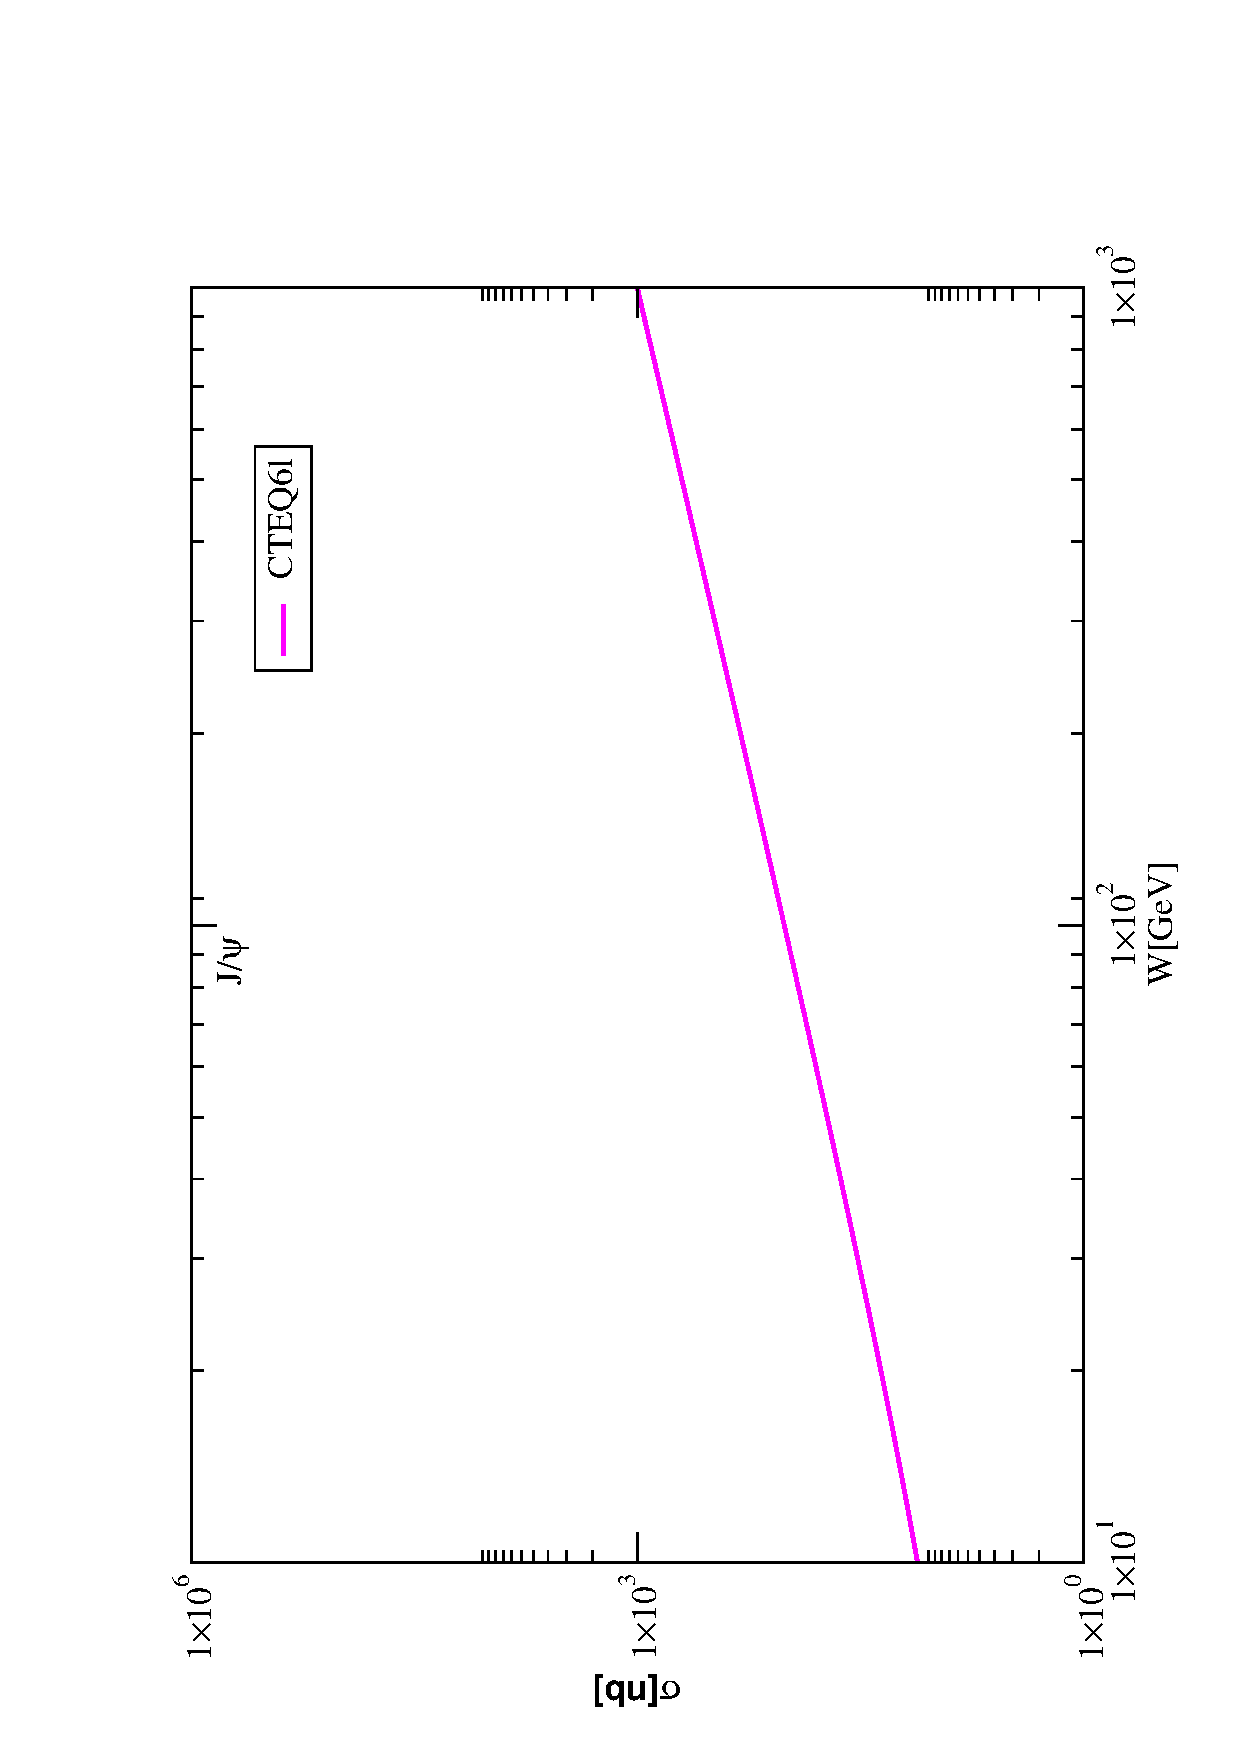
\includegraphics[width=.5\linewidth]{img/plot-J_psi.png}
						\caption{Seção de choque total para $J/\psi$ em função da energia do centro de massa tomando por referência os parâmetros estudados em \cite{LUIS:2014}.}
					\end{figure}
				}
				\only<2>{
					\begin{figure}[htb!]
						\centering
						\includegraphics[width=.8\linewidth]{img/plot-J_psi-Luis.png}
						\caption{Seção de choque total para $J/\psi$ em função da energia do centro de massa com $b_{V}=4,5\; \mathrm{GeV}^{2}$ e $\alpha_{s}-0,20$ fixos para $\mu^{2}=2,4\; \mathrm{GeV}^{2}$ e $\mu^{2}=9,0\; \mathrm{GeV}^{2}$ respectivamente.}
					\end{figure}
				}
			
			
				
			\end{frame}

			% --------------------------------------------- %
			\begin{frame}[allowframebreaks]
				\frametitle{Referencias}
				\bibliography{referencias.bib}
			\end{frame}

			\contato{%
				Contato: \\
				\autor{} \\
				\email{} \\
				\github{} \\
				\website{}
			}

			\capadetras{}

			\end{document}
